\documentclass[12pt]{article}
\usepackage{amsmath}
\usepackage{graphicx}
\usepackage{hyperref}
\usepackage[utf8]{inputenc}
\usepackage{listings}
\graphicspath{ {./SampleImages/} }

\title{CSU44053 Computer Vision}
\author{Draughts Video and Image Processing \\ Daniel Whelan \\ 19335045}
\date{02/11/2022}


\begin{document}
\maketitle
\newpage

    \section*{Question Statement}
    You are asked to develop a system to automatically analyse a game of draughts (also known as checkers).
    \begin{center}
        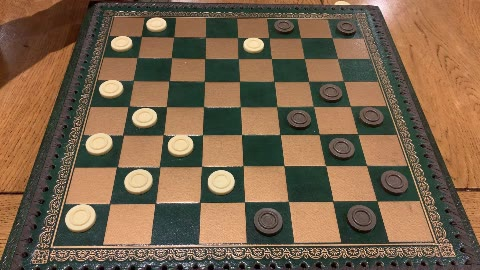
\includegraphics[scale=0.5]{DraughtsGame1Move13.png}
    \end{center}
    As this assignment was released in five individual parts, this report will follow a similar structure, handling each part in its own section.
    \newpage
    
    \section{Part 1 - Pixel Classification}
    \subsection{High Level Overview of Problem Statement}
    It was asked that we develop an application that classified all pixels in the image as:
    \begin{itemize}
        \item Part of a White Piece
        \item Part of a Black Piece
        \item Part of a White Square
        \item Part of a Black Square
        \item None of the above
    \end{itemize}
    \subsection{Processing of Image}
    \par
    To describe the process of detecting what section pixels belong to, I will describe the process of detecting a single section, the detection of White Pieces.
    \par
    Firstly. I converted the initial image of a draughts board and pieces and sample image of the white pieces from a BGR (Blue, Green, Red) image to a HSV (Hue, Saturation, Value) image. 
    Following this I created a histogram representation of the HSV sample image, displaying the intensity of the three channels (HSV) in histogram format, and used this to perform a Back Projection onto the initial image.
    From this, I was output a Probability image of the likelihood of a pixel being part of a White Piece. I then converted the HSV Probability Image to a Greyscale image and perfromed a Binary Threshold using a fixed threshold of 100,
    giving me a Binary Image representation of the Probability Image. I then perfromed some Mathematical Morphology operations on this image, first a closing operation and then an opening operation, in order to gain a more accurate
    representation of what pixels belonged to White Pieces. Finally, on this Morphed Binary Image I performed a Connected Components Analysis (CCA) in order to determine where the regions that belonged to white pieces were.
    This returned an image with the pixels that belonged to a white piece coloured white.
    \par
    The same steps were performed for each of the other sections, with different colours used to represent different sections. 
    \newpage
    \subsection{Results}
    \begin{figure}
        \begin{minipage}[c]{0.4\linewidth}
            \centering
            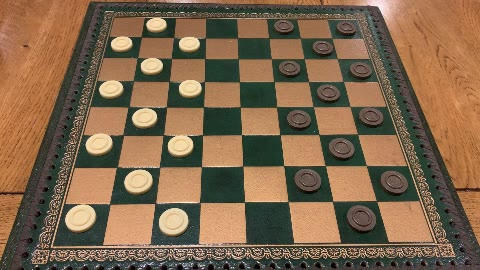
\includegraphics[width=6cm]{DraughtsGame1Move0.png}
            Original Image
        \end{minipage}\hfill
        \begin{minipage}[c]{0.4\linewidth}
            \centering
            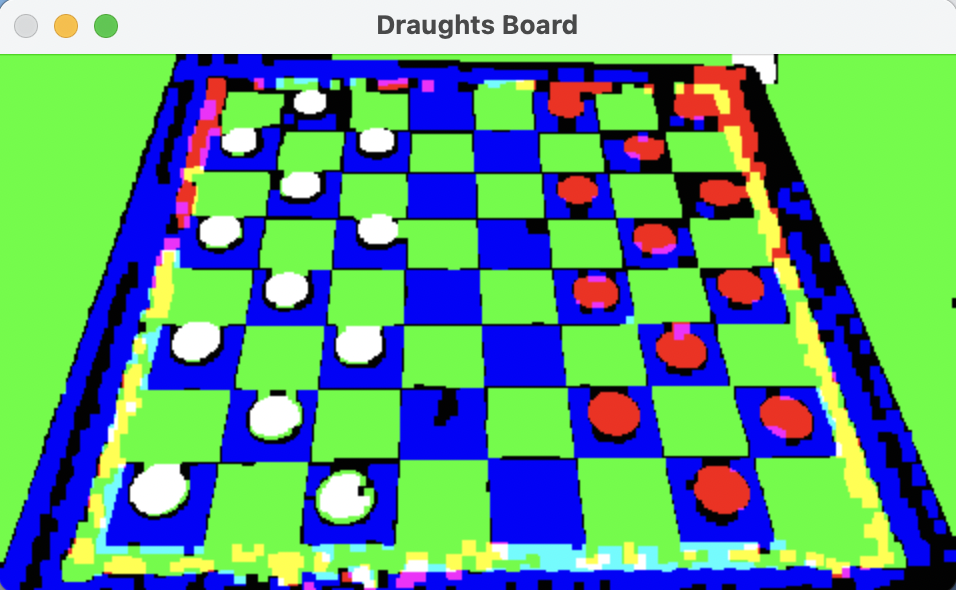
\includegraphics[width=6cm]{HSV-Combined-Image.png}
            HSV Result Classification
        \end{minipage}\hfill
        \begin{minipage}[c]{0.4\linewidth}
            \centering
            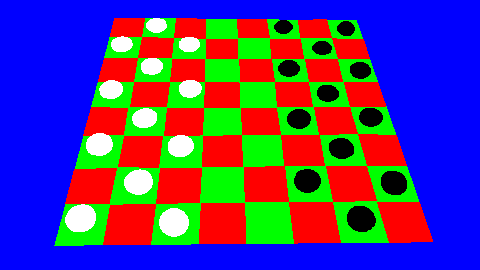
\includegraphics[width=6cm]{DraughtsGame1Move0GroundTruth.png}
            Ground Truth Classification
        \end{minipage}
        \caption{Result vs. Ground Truth and Original Image}
    \end{figure}
    \par
    As can be seen above (Figure 1), this process has accurately identified a number of pixels. The White Pieces \emph{(White)} and the White Squares \emph{(Green)} are very clearly identifiable. Also in a large number of places
    The Black Pieces \emph{(Red)} and Black Squares \emph{(Blue)} have also been correctly identified, apart from certain areas of the image where it is possible to see that the pixel classification has been distorted by noise 
    (Often the brightness/shadows present in the image).
    \par
    However, This is not perfect as It can be very clearly seen that the wooden edging around the  board has in parts been classified as nothing \emph{(Black)} but has also been classified as a Black Square. Similarly, all of the table
    around the board has been classified as a White Square, which highlights an issue with the overall classification of pixels in the image, with a large number of the unimportant edging pixels being classified as important object pixels.
    \par
    In conclusion, Although the actual region detection of the board and its important objects (White Pieces, Black Pieces etc) has been handled quite well by the process, The overall pixels outside of the playing board have been 
    for the most part misclassified, and improvement is needed in this area.

    \newpage
    \subsection{Comments and Final Remarks}
    \par
    As discussed previously, there are some issues with the overall classification of unimportant pixels and this would need improving going forward. One way in doing this would be to gather a larger collection of samples for each section
    That we are looking for, and possibly remove some issues that may be present in these samples, for instance, the sample images taken for the white squares (Figure 2) contains a darker colour that is not necessarily representative of the
    regions we are attempting to classify, as a result, this possibly led to the brown table the board is resting on being classified as a "White Square".
    \begin{figure}
        \centering
        
\includegraphics[scale=1]{DraughtsGame1WhiteSquares.png}
        \caption{White Square Sample Images}
    \end{figure}
    \par
    Following this, for images with poor lighting this process will not work as the Probability Image produced from Back Projection may fail to discover any regions that have a similar HSV histogram to the Sample Images, and this would only be
    rectified by adding additional sample images specific to that lighting scenario. In Essence, This process may not work in a general context due to good lighting conditions being required. Following this, Equalisation is not a vaid way of solving
    this issue as this alters the Histogram of the initial image and hence any Back Projection using sample images will not return an accurate Probability Image.
    \par
    As a final remark on this part of the assignment, I feel that my method of classifying pixels was very effective when focusing only on the draughts board and successfully identified pixels that belonged to the different regions we were looking for.
    However, when it came to classification outside of the board, the process failed to classify pixels that were unimportant (\emph{None of the Above}) and hence the overall process, whilst successful in parts, overall returned middling results regarding classification.
    One way to possibly improve this is to also take sample images of the areas outside of the board (table, frame etc) and do some analysis to confirm they are present and hence classify the regions correctly.
    
    \newpage
    \section{Part 2 - Piece Detection}
    \subsection{High Level Overview of Problem Statement}
    \par
    Given the four corners of the board, Determine whether there is a piece on a square and what kind of piece that is (White or Black)

    \subsection{Determining Pieces on Squares}
    \par
    Firstly, given the four corners of the board it was possible that, when given an RGB image of the board, a perspective transformation could be done that removes the areas surrounding the board (table, frame, etc) and placing the board in a 400px x 400px Matrix. Following this the processing outlined in "Part 1" was
    performed on the newly transformed image, giving CCA images for each pixel class (See Below).
    \begin{center}
        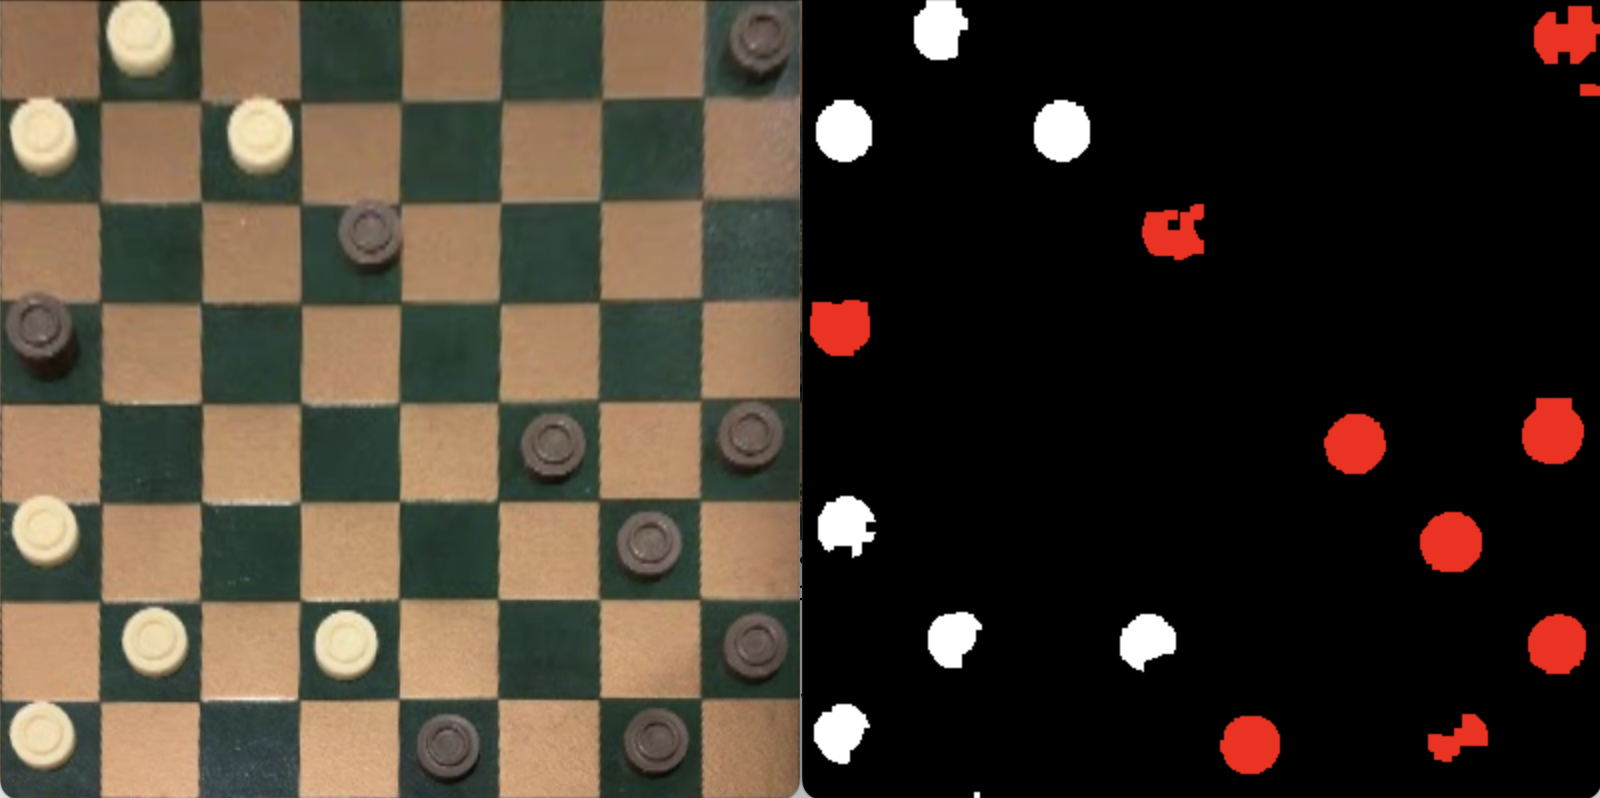
\includegraphics[scale=0.25]{TransformedAndPieces.png}
        \newline
        Transformed Image and Pieces Detected
    \end{center}
    \par
    Following this, I performed some cleaning of the region detection by determining whether the area classified as a certain pixel was part of that class. For example, some pixels were wrongly classified as \emph{White Pieces} when they should not have been. To do this, a 
    comparison was done between the CCA matrices to determine whether a pixel classified as a \emph{White Piece} was also detected resting on a \emph{Black Square}. By doing this a large number of pixels that had been incorrectly classified were corrected (Figure 3).
    \par
    Furthermore, I initialised a Portable Draughts Notation (PDN) Matrix in order to number the pieces that had been detected on playing squares. The actual detection of pieces was done by determining the center point of a square (Being the number of pixels in the transformed column
    divided by the Number of playing squares on each side), and seeing whether this center point was classified as both a Piece and a Playing Square, and hence storing this piece in the PDN matrix.   

    \newpage
    \begin{figure}
        \centering
        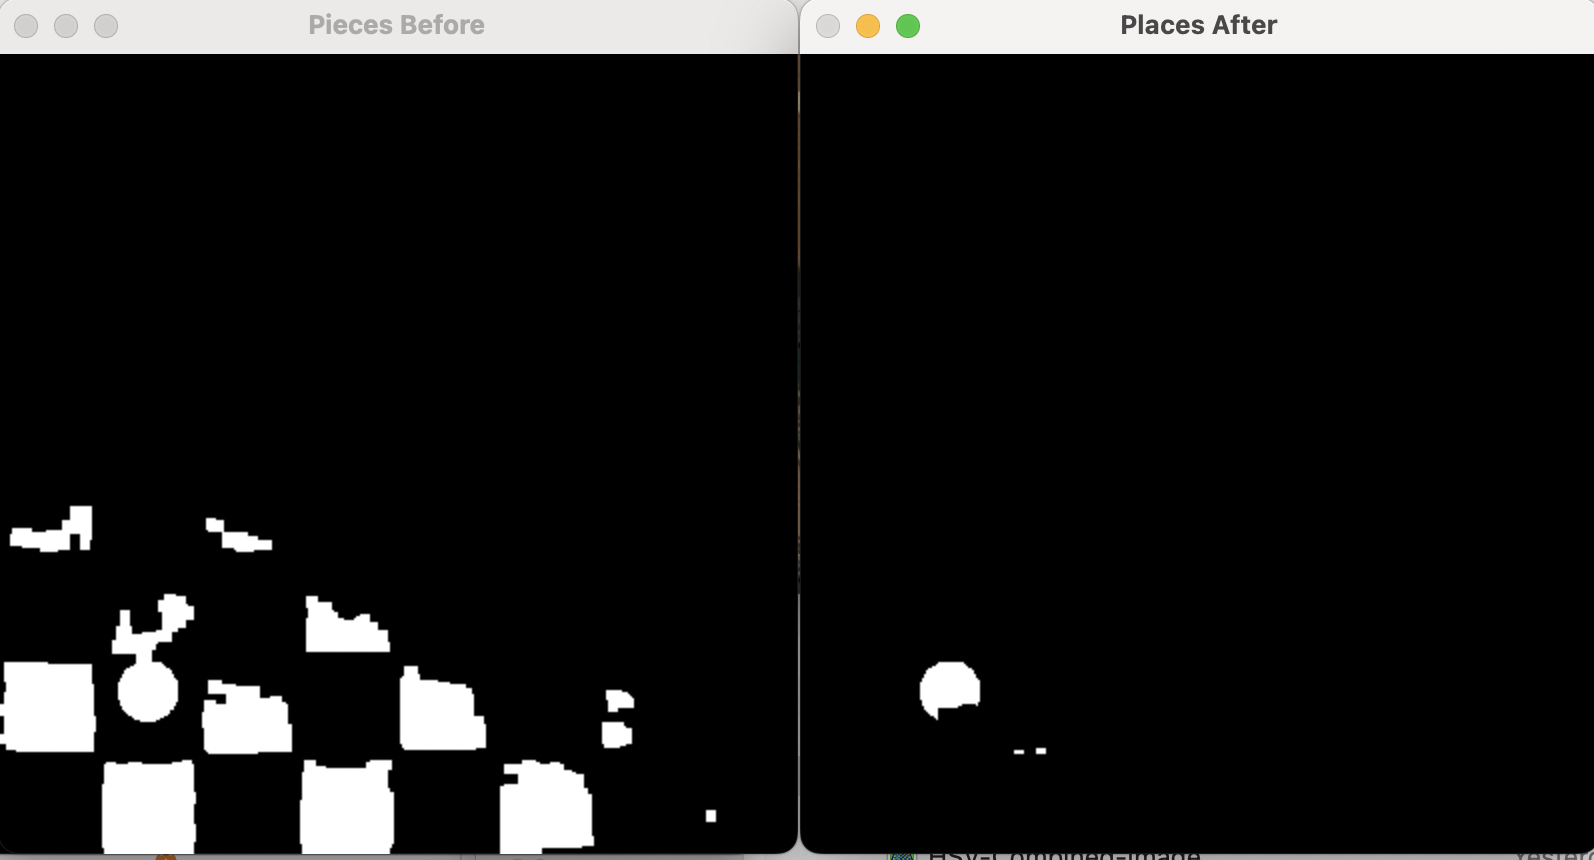
\includegraphics[scale = .3]{Bad-v-Good-piece-detection.png}
        \caption{Detection Before vs Detection After Classification Cleanup}
    \end{figure}

    \subsection{Results}
    \par
    Overall, this process performed much better than the previous part. When comparing the results to the Ground Truth Provided for the 69 Static Images, this processing had a Successful Detection Rate of 97\% giving 753 True Positive detections (i.e A piece was detected and also a piece was
    expected to be present) and 66 False Positive detections (i.e A piece was detected but no piece was expected to be present). There were also no False Negative (i.e No piece detection and piece present) detections and 1,389 True Negative detections (i.e No Piece Detected and No piece expected 
    to be present, An Empty Square).
    \begin{center}
        
\includegraphics[scale=1]{AssignPt2Res.png}
        \newline
        Ground Truth Comparison Results
    \end{center}
    \par
    This small number of False Positive detections highlights that the process is running as expected and to a high level. Some of the false positives have come from the incorrect classification of pixels by the process outlined in part 1, misclassifying certain squares as pieces due to possible 
    changes in lighting, or shadows present in the scene (See Below).
    \begin{center}
        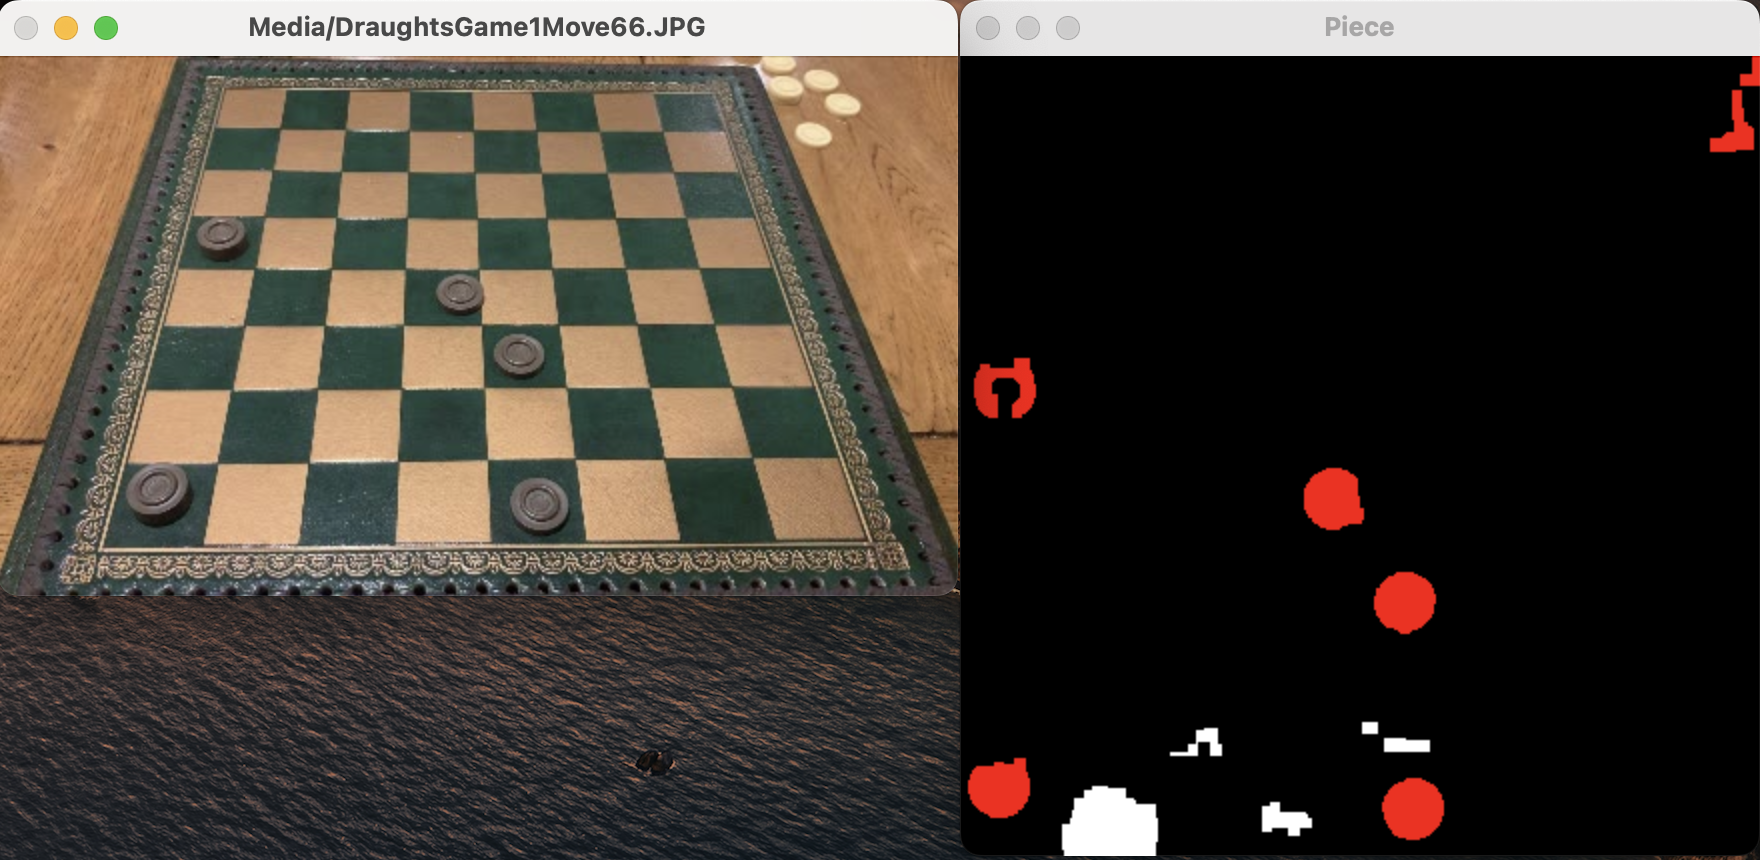
\includegraphics[scale=0.2]{FPExample.png}
        \newline
    \end{center}

    \begin{figure}
        \begin{minipage}[c]{0.4\linewidth}
            \centering
            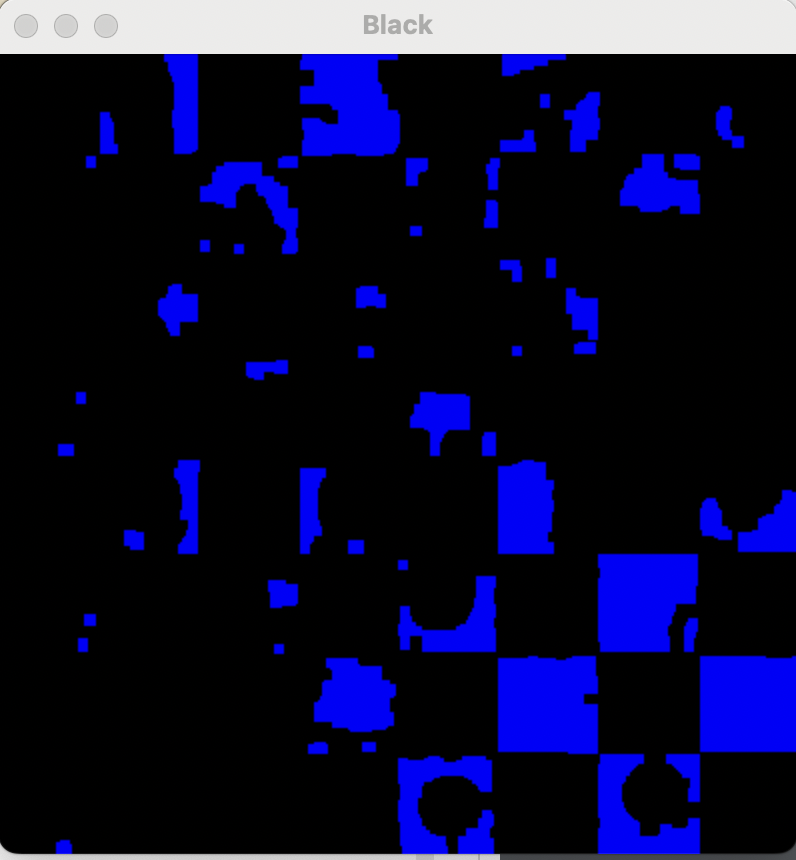
\includegraphics[scale=0.3]{Bad-Black-Squares.png}
            \newline
            Poor Classification
        \end{minipage}\hfill
        \begin{minipage}[c]{0.4\linewidth}
            \centering
            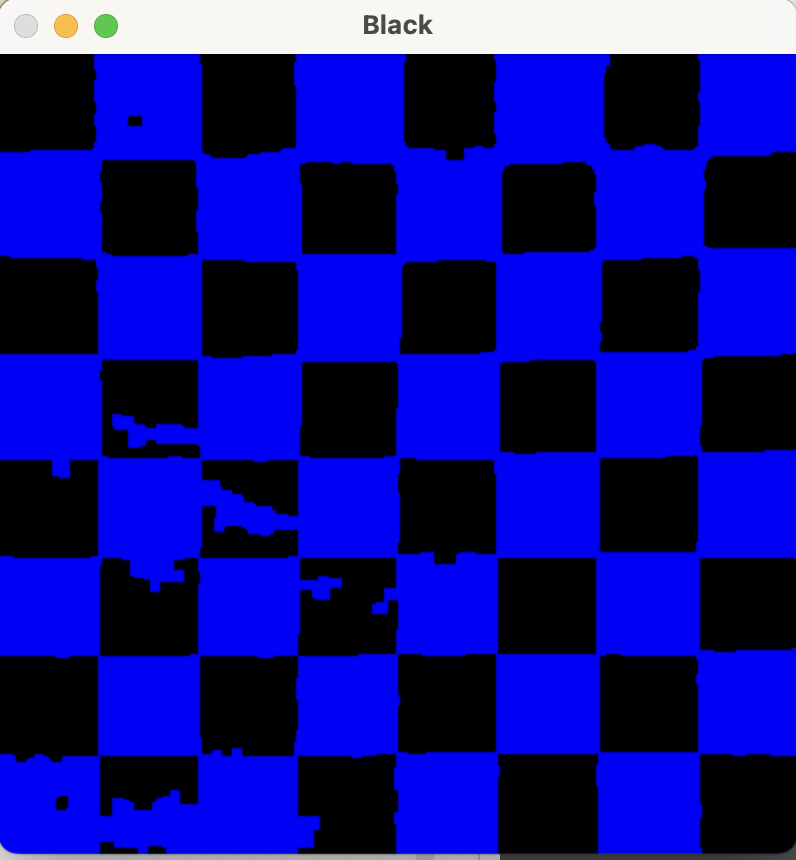
\includegraphics[scale=0.3]{Good-Black-Squares.png}
            Cleaned Classification
        \end{minipage}
        \caption{Improving Classification}
    \end{figure}
    \subsection{Comments and Final Remarks}
    \par
    As can be seen by the results of this part Piece Detection and numbering based on the PDN system was very successful. This is thanks in part to cleaning the classification of pixels received
    from processes in part 1. As can be seen in Figure 4, cleaning the classification of these squares was a massive advantage in determining the position of pieces on the board. This is particularly
    true for black piece and square classification as due to lighting and shadows in the images, performing BackProjection resulted in receiving inaccurate probability images for these regions. However, by
    using the information received via the probability images of their white counterparts, it was possible to improve the classification of these pixels, as can be seen above.
    \par
    Furthermore, the use of the center of squares as a point of reference for determining whether a piece was present or not also led to an efficient program as there was no processing of entire squares 
    (reducing the pixels checked per square from 2,500 [\((\dfrac{400}{8})^2\)] to 1). This also improved detection accuracy as it is most likely that the piece, when placed, will in some way or another cover 
    that center pixel.
    \par
    Overall, I feel that this part of the assignment strongly detects pieces and correctly places them on a PDN representation of the board with a strong level of accuracy. 

    \newpage
    \section{Part 3 - Video Processing}
    \subsection{High Level Overview of Problem Statement}
    \par
    Process a video of a draughts game identifying appropriate frames to process (Without using the Static Images Provided). Find and record moves again using the PDN notation.

    \subsection{Video Processing}
    \par
    With the input of an RGB video I did a similar initial process to thise of the static images and performed a Perspective Transformation using the given corners to remove any external information not relevant to the
    draughts game (table, frame etc.). Following on from this, I applied the Gaussian Mixture Model (GMM) creating a foreground mask for the frame, which I then performed a Binary Threshold with a high fixed threshold of 150 on
    in order to remove any noise from this mask. Furthermore, I then applied some Mathematical Morphology operations to this thresholded image using a 3x3 structuring element, performing a closing operation followed by an opening
    operation in order to get a more accurate representation of where the moving object pixels are present.
    \par
    With this Binary Moving Object image, I then counted the number of white pixels (i.e moving) that were present in the frame and ratioed this against the total number of pixels present in the frame. If this ratio was smaller than
    the fixed tolerance of 3\%, and only after being higher than the tolerance in the frames just previous, this frame would be analysed and the system would then wait for the ratio to become higher than this tolerance again before allowing
    another frame to be analysed.
    \par
    In essence, the main functionality of this process is to wait until the number of moving object pixels has dropped below a certain tolerance level then, and only then, analysing a frame of the video.
    \begin{center}
        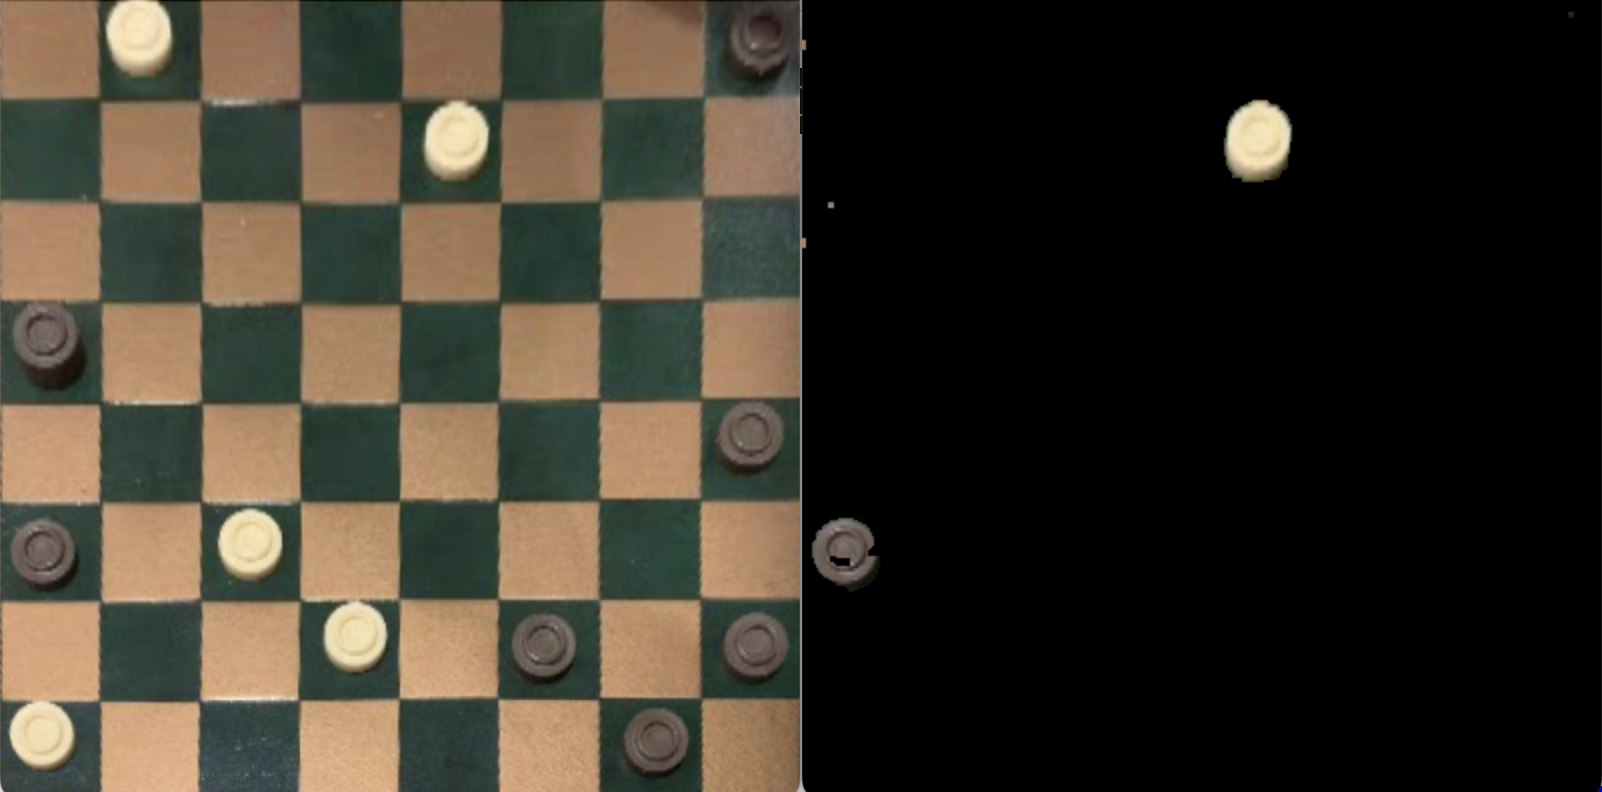
\includegraphics[scale=0.21]{GMMEg.png}
        \newline
        Example of GMM in use
    \end{center}

    \newpage

    \begin{figure}
        \centering
        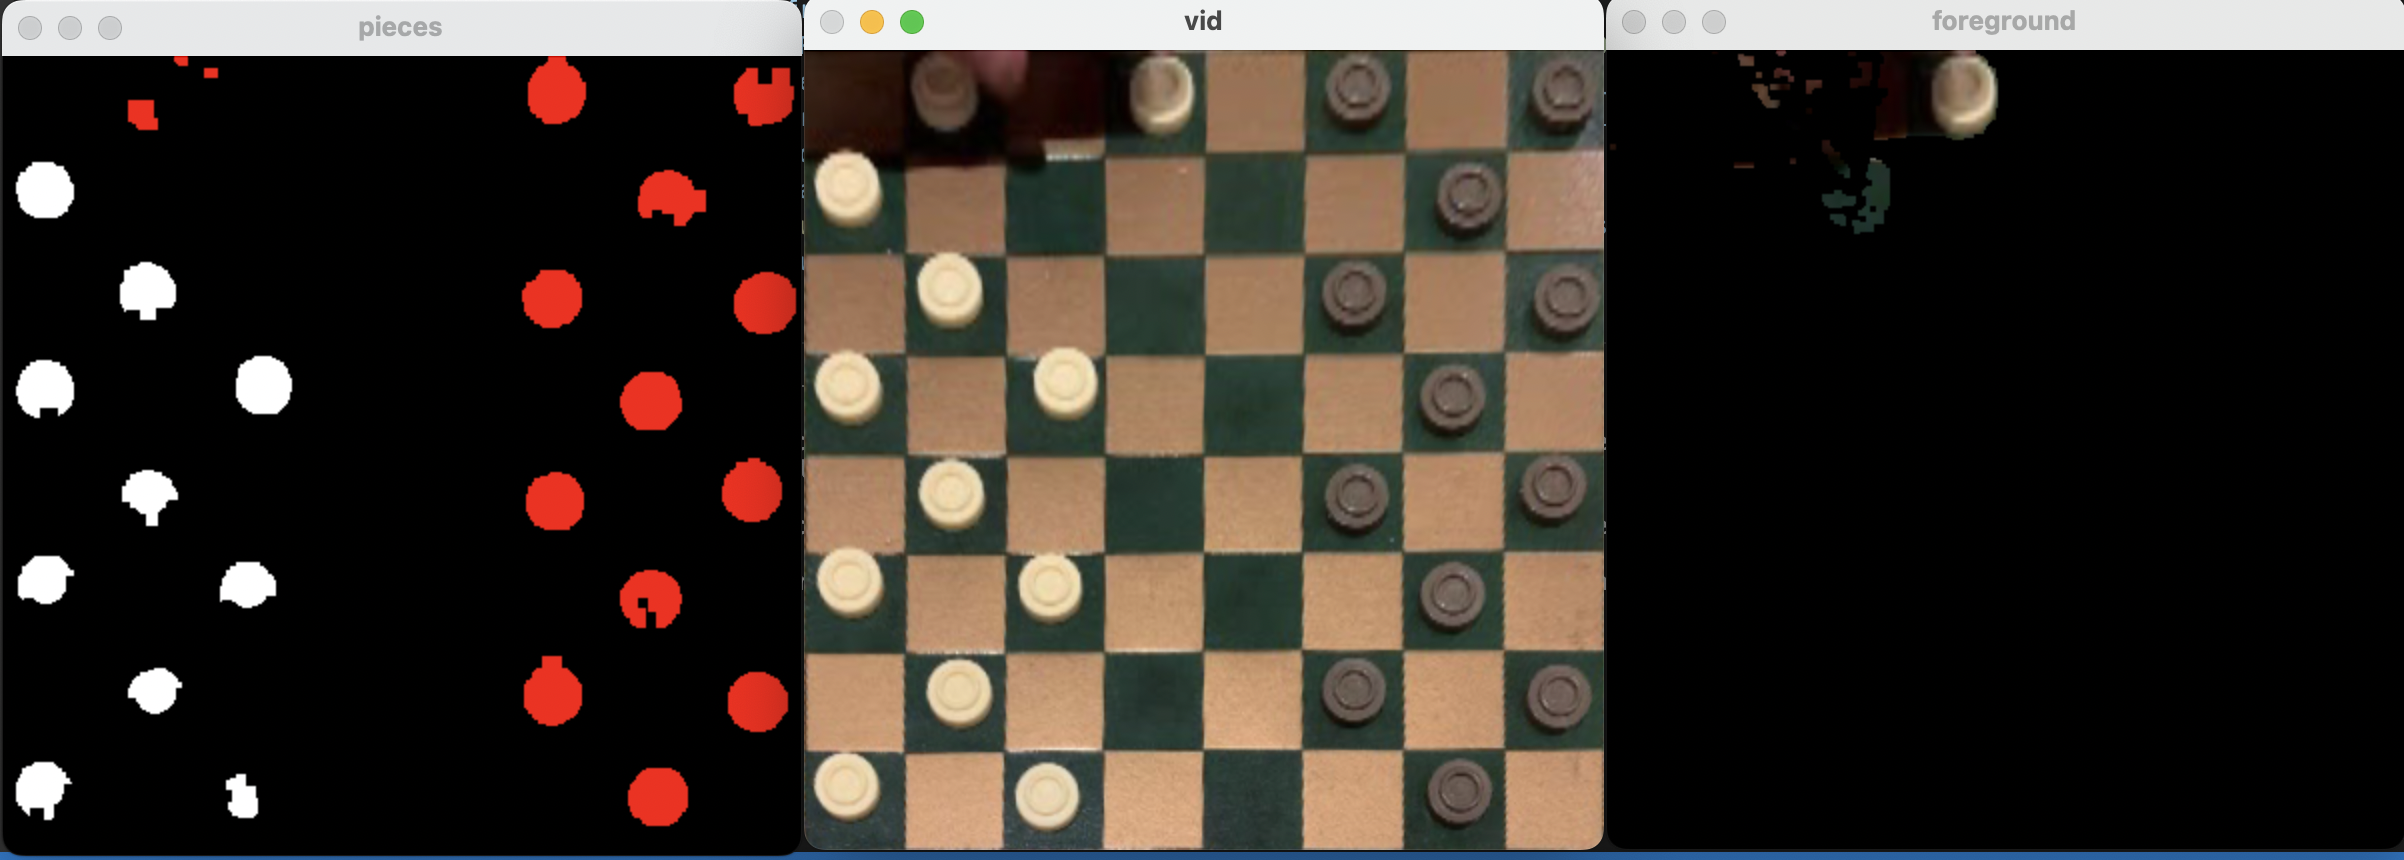
\includegraphics[scale=0.3]{Shadow-Covering-Pieces.png}
        \caption{Shadows Effecting Move Detection}
    \end{figure}

    \subsection{Results}
    \par
    The process described above identified 76 frames that it deemed were appropriate for analysis. This is an 11\% increase on the Ground Truth value of 68 frames. Within that 76 frames however, all 68 frames from the ground truth were either identified exactly or were 
    \(\pm\) 5 frames from the Ground Truth frame identified. This highlights that the method of determining moving object pixels under a certain tolerance was an effective process for determining frames to analyse.
    \par
    Following from this, the number of moves detected by the processes outlined in part 2 had a success rate of 84\%, detecting 57 of the total 68 moves made during the video. Whilst I would've preferred a higher success rate, I feel that 
    the process detects the vast majority of the moves made.
    \begin{center}
        
\includegraphics[scale=1]{AssignPt3Res.png}
        Ground Truth Comparison Results
    \end{center}
    \par
    As can be seen in Figure 5, one of the main issues for moves not being detected was that at certain frames that were chosen for analysis, there was a small possibility that the pieces of interest were covered by a shadow
    and as a result, this has effected the pieces being detected in this frame. You can see, the piece that has been moved has not been detected by the processes mentioned in Part 2, and furthermore, a piece in square 5 (PDN) 
    has in fact been identified as a black piece by Back Projection.
    
    \newpage

    \begin{figure}
        \centering
        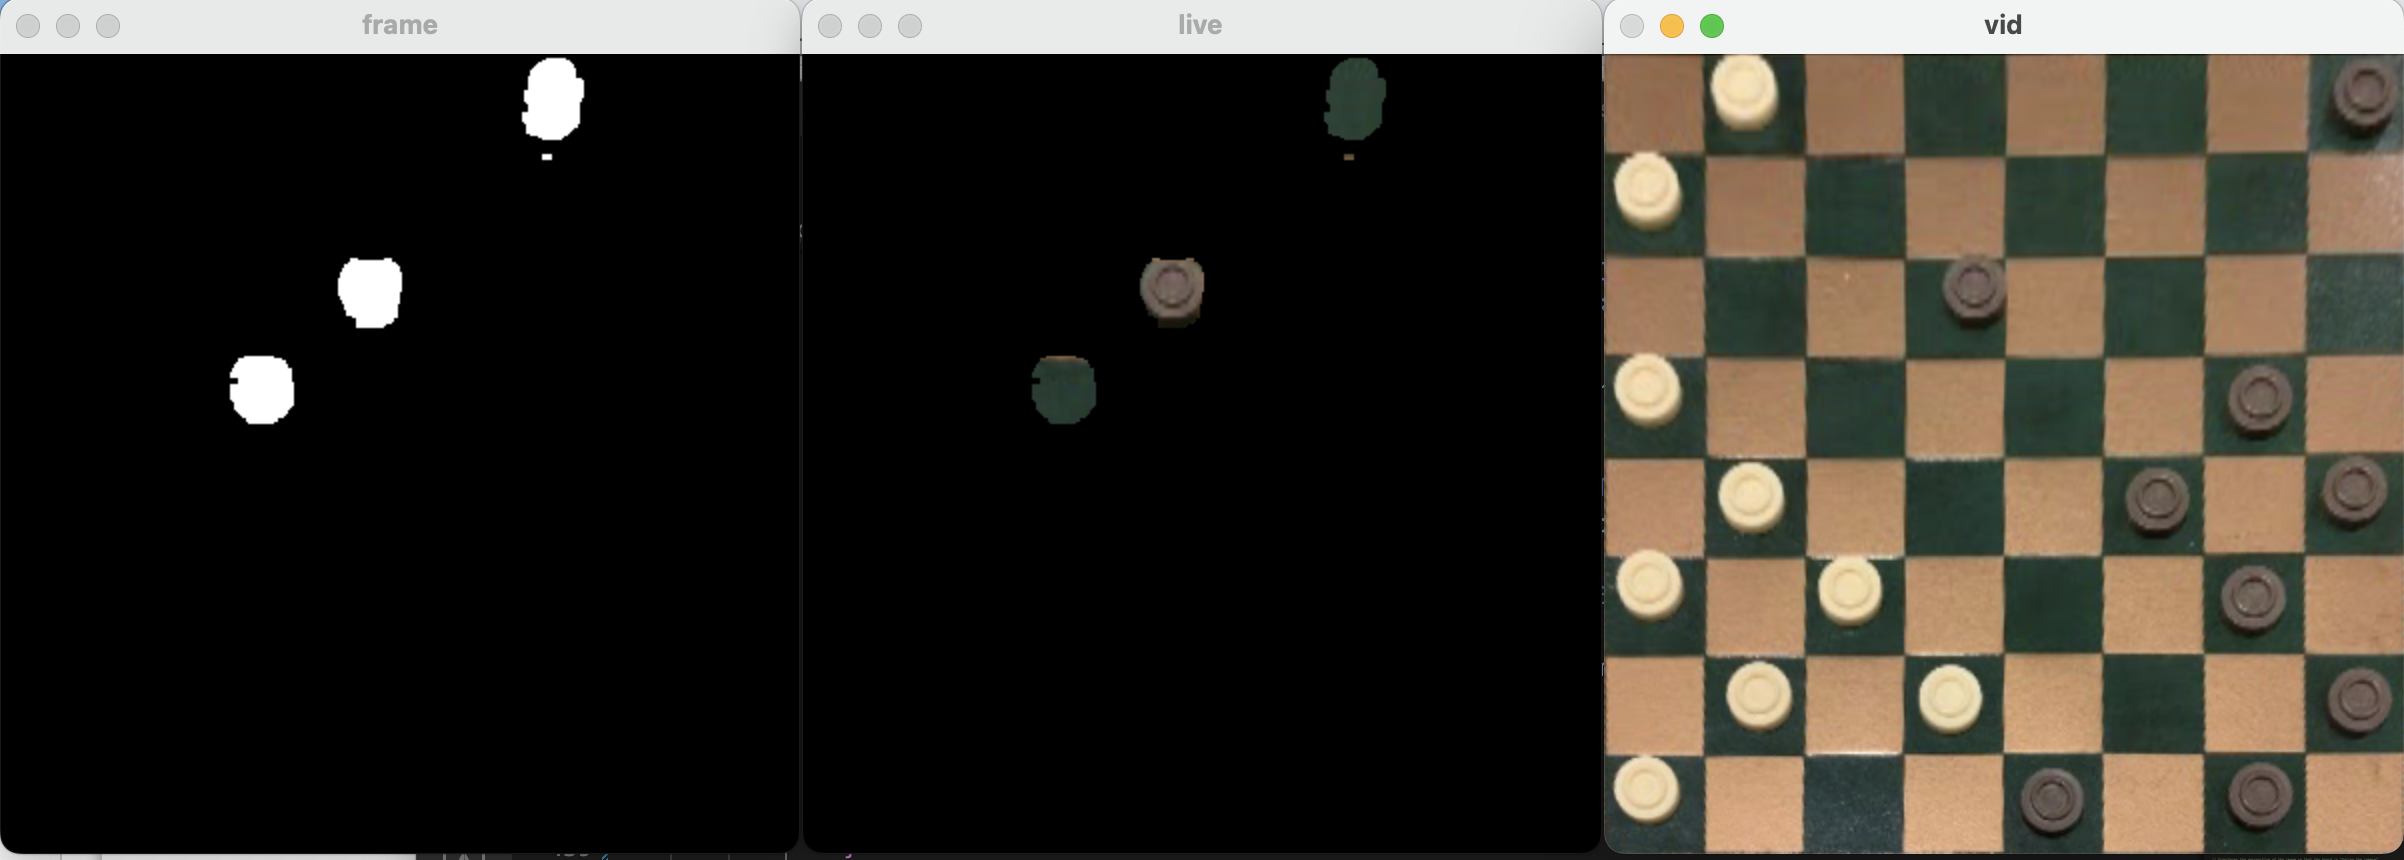
\includegraphics[scale=0.3]{Poor-Detection.png}
        \caption{Poor Background Modeling}
    \end{figure}

    \subsection{Comments and Final Remarks}
    \par
    From the results previously shown, it can be seen that this way of processing video is very successful and is able to appropriately detect frames to analyse, and also detects a large number of moves. However there are some 
    issues that should be addressed
    \par
    Firstly, As shown previously in Figure 5 pieces that have been covered by a shadow are difficult to detect, and one way around this could be to analyse the frames that come directly after it in order to see if a piece has been
    misclassified. However, this requires a knowledge of the exact game that is being played, possibly via ground truth analysis, and obviously is not an effective solution in a general system that is analysing draughts games.
    \par
    Another issue comes from the background model. As can be seen in Figure 6, the background model has seen two pieces been moved from their spaces and has left two holes in their places. From a qualitative analysis by myself, this 
    issue persists for a long period of time until the model "dissolves the moving object pixels" into the background. If this were to happen for a large number of moves rather than just two pieces, it could be observed that frames 
    would no longer be selected for analysis as the number of moving object pixels as increased over the tolerance. A way of possibly fixing this is by increasing the learning rate of the Gaussian Mixture Model used and this would perhaps 
    allow for a quicker dissolution of "old" moving object pixels.
    \par
    Overall, I would say the processes used for this part of the assignment have been a success and provide an accurate representation of the moves made during the video of a draughts game.

    \newpage
    \section{Part 4 - Edge and Corner Detection}

    \subsection{High Level Overview of Problem Statement}
    \par
    Process any static image of the board and attempt to determine the locations of the four corners, compare the following approaches:
    \begin{itemize}
        \item Hough Transformation for Lines spanning the complete image
        \item Contour Following and Line Segment extraction
        \item Use of the \emph{findChessboardCorners()} in OpenCV
    \end{itemize}
    \subsection{Hough Transformation for Lines Method}
    \par
    Firstly using a Greyscale image of the playing board with no pieces, a Canny Edge detection was performed in order to get a Binary Edge Image of the board. Following this, a Hough Transformation for lines was done. This returns a series of lines in \(\rho,\theta\) form.
    Following this I did a k-means clustering in order to determine lines that were vertical and those that were horizontal, multiplying \(\theta\) by 2 in order to bring the lines closer to their exact orientation (as numbers close to 0/360 and 90/180 may confuse the algorithm
    as to which orientation they belong). Although I did not manage to finish this implementation the following steps would be; I would find the intersections between lines of different orientations and in order to find the corners I would determine points with a large euclidean 
    distance between end points. Finally I would use these points to determine the corners of the playing board.
    \begin{center}
        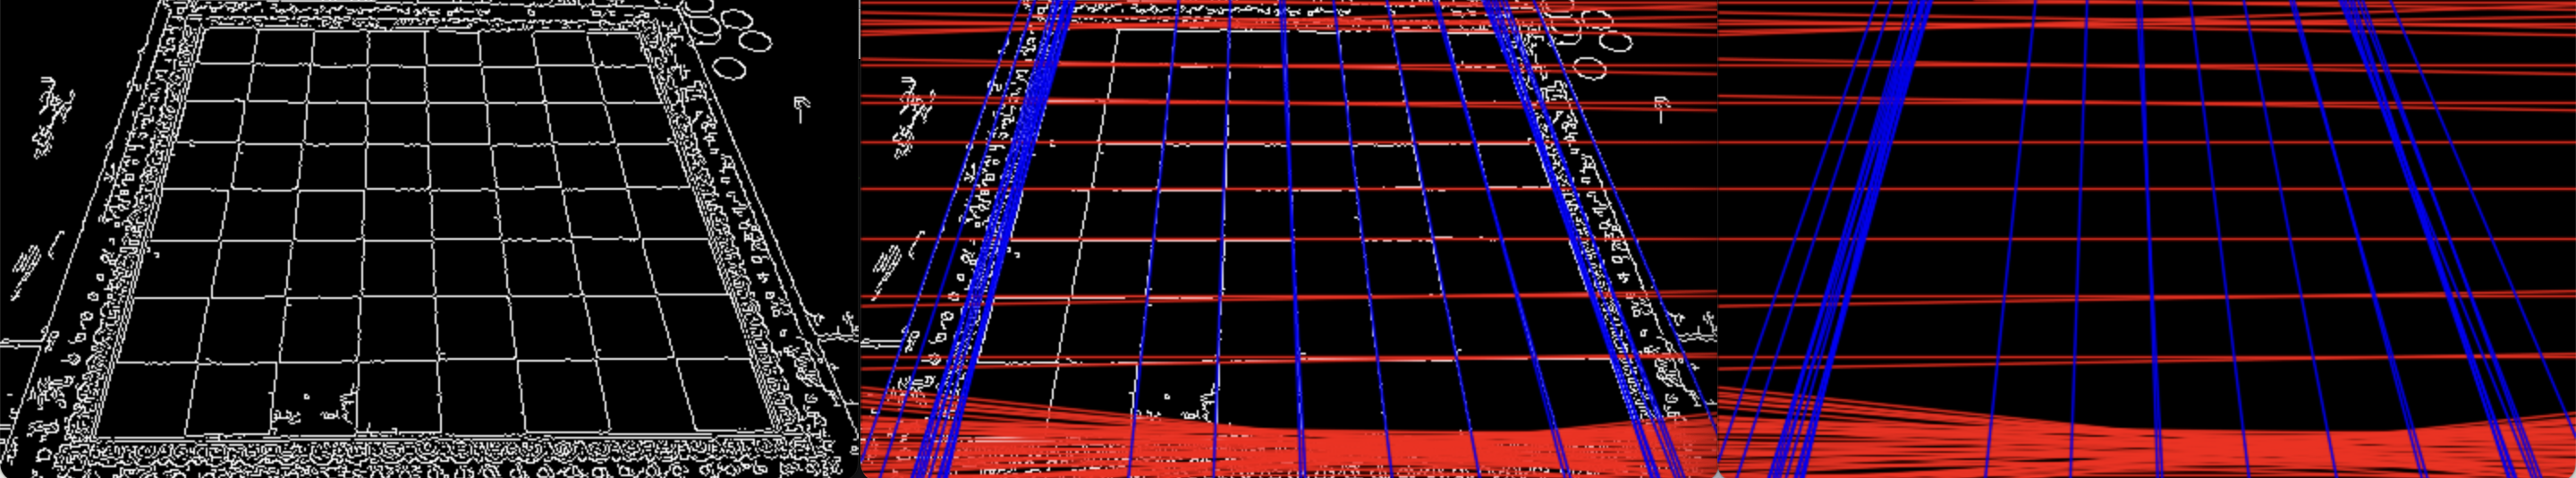
\includegraphics[scale=0.3]{HoughLines.png}
        Binary Edge Image and Hough Lines Image
    \end{center}
    
    \newpage
    \subsection{Contour Following and Extracting Line Segments}
    \par
    Similarly to the Hough Transformation, I did a Canny Edge Detection on a Greyscale image of the board and received a Binary Edge Image. Following this I determined the contours present in this image and a series of Boundary Chain Codes were obtained. From these I was then able to 
    extract Line segments from this using Contour Segmentation. Following this, I would have detected interections in the line segments and looked for line segments that rest on a similar angle to other segments in order to create larger segments. Once this was finished I would, as above,
    determine lines with a large euclidean distance between end points and from this determine the corners of the playing board.
    \begin{center}
        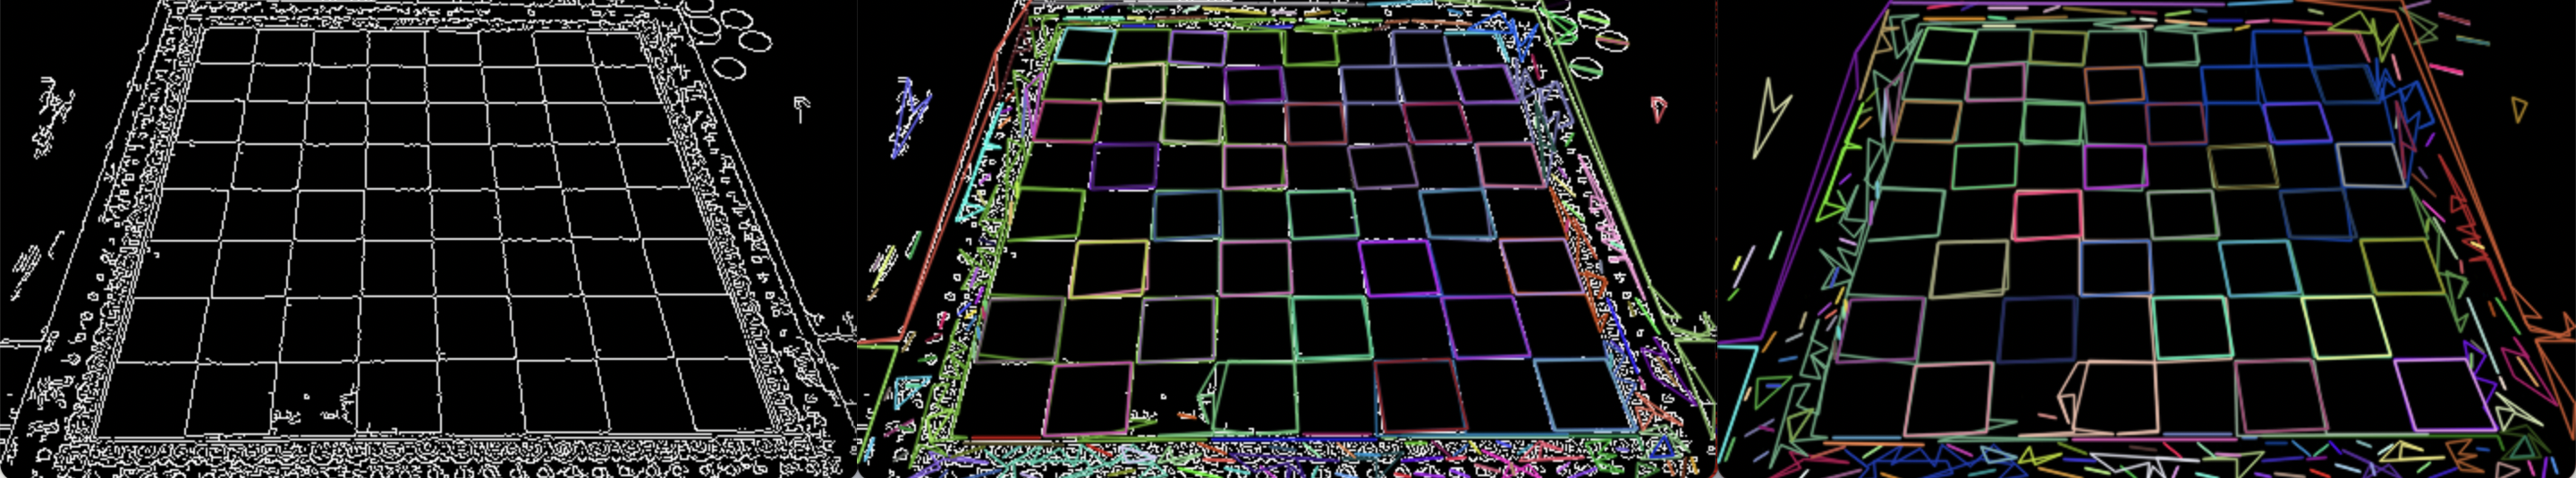
\includegraphics[scale=0.3]{LineSegments.png}
        Binary Edge Image and Line Segments Detected
    \end{center}

    \subsection{\emph{findChessboardCorners()}}
    \par
    the \emph{findChessboardCorners()} function in OpenCV is used when calibrating cameras. The function takes in a Greyscale image (and if colour, converts to Greyscale) that may or may not contain a checkerboard pattern and returns true if one is detected and false if not. It also returns a vector of internal corners that the 
    function has detected in the checkerboard pattern. The algorithm converts the Greyscale image to a Binary Image and then thresholds with a high fixed threshold to make an extreme distinction between white squares and black squares. The Binary Image is then dilated in order to separate the squares and split the corners apart.
    The algorithm does this dilation multiple times as some squares do not split properly with one dilation. However, the image cannot be dilated too much as squares reduce in size each time and become too small to detect. The algorithm then detects the squares using Contour Following and then uses the points at which there are 
    two extreme gradients meet going in different directions. It then cleans the number of corners detected based on a checkerboard pattern and returns all of the detected corners (Figure 7).
    
    \begin{figure}
        \centering
        \includegraphics[scale=0.25]{findChessboardCorners.png}
        \caption{\emph{findChessboardCorners()} Result (7x7)}
    \end{figure}

    \subsection{Comments and Final Remarks}
    \par
    Each of these methods allow for the location of the chessboard corners. However, some will work in a more accurate way than others. The Hough Transformation for Lines allows for easy detection of lines, their orientation and intersection points, however, As can be seen in the Hough Lines image, a large number of "noisy" lines 
    are also detected making it difficult to determine which intersection points may be corners and which are irrelevant. A RANSAC algorithm may help reduce this in normal instances but due to the ornate frame of the board in this particular instance it may only remove a small number of unimportant lines. 
    \par
    Comparing this to the Line Segment Extraction from finding Contours, This returns a large number of small lines, that could be used to detect squares and in turn follow a similar algorithm to that of \emph{findChessboardCorners()}, but again in this instance, the board frame causes issues creating unimportant line segments and makes
    the edge detection "noisy". 
    \par
    Using \emph{findChessboardCorners()} returned an accurate depiction of the corners present internally in the chessboard. However, this used a Search size of 7x7 rather than 8x8, which would be required for this board. Again, the frame of the board causes issues for this function as, according to OpenCV documentation,\emph{"The function requires white space
    around the board to make the detection more robust"} as a dark border causes the external black squares to be segmented incorrectly and hence fails to detect the corners correctly.
    \par
    Overall, when detecting the checkerboard corners, One could combing the Hough Transformation for Lines, with the Line Segments detected to remove noise and then check intersections and euclidean distances of Hough Lines to get accurate 
    corners of the board.

    \newpage
    \section{Part 5 - Detect King Pieces}
    \subsection{High Level Overview of Problem Statement}
    \par
    Develop Code to distinguish between normal pieces and King pieces.

    \subsection{Processing King Pieces}
    \par
    




\end{document}
